\chapter{Connect Model to Libraries}
We store the information of a higher-order linear ODE in the \verb|DifferentialModel| in Chapter 2. This \verb|data type| captures the structure of the ODE so that we can transform the ODE into other forms. Chapter 3 discusses how to solve a system of first-order ODEs numerically in four selected external libraries. However, there is a gap between the \verb|DifferentialModel| and external libraries. The selected libraries cannot solve the higher-order ODE directly, but they can solve its equivalent system of first-order equations. We know that most ways of solving ODEs are intended for systems of first-order ODEs, so we want to convert the higher-order ODE to a system of first-order ODEs~\citep{converthigherode}. Firstly, we transform a linear higher-order ODE into a system of first-order ODEs. Then, we use the Drasil Code Generator to generate code that contains proper interfaces for utilizing four selected external libraries. This program solves the system of first-order ODEs numerically by producing a list of values of dependent variables based on time. The original linear higher-order ODE is equivalent to the system of first-order linear ODEs we solve. Thus, by transitivity, the numerical solution for the system of first-order ODEs is also the numerical solution of the higher-order ODE.

In this research, my work primarily focuses on enabling the Drasil Code Generator to generate code for solving higher order ODE and automatically extracting useful information from \verb|DifferentialModel| for the Drasil Code Generator. In addition, we create a new case study, Double Pendulum, which has a system of non-linear ODEs. We handle the nonlinear ODE different than the linear ODE. The nonlinear ODE still requires Drasil users manually extract information from the original ODE. With the new implementations, we can to generate code to solve the Double Pendulum numerically. In this chapter, we will first discuss how to convert any higher-order linear ODE to a system of first-order ODEs in theory. Then, we will discuss how to enable the Drasil Code Generator to generate code that produces a numerical solution for a system of first-order ODEs. Lastly, we will discuss how to automate the generation process.

\section{Higher Order to First Order}
\label{se_hightofirst}
Any higher-order linear ODE can be written in the following form:
\begin{equation} \label{eq_isohighode}
  y^n = f (t, y, y', y'', \dots, y^{\textit{(n-1)}})
\end{equation}

We isolate the highest derivative $y^n$ on the left-hand side and move the rest of the terms on the right-hand side. On the right-hand side, $f (t, y, y', y'', \dots, y^{\textit{(n-1)}})$ means a function depends on variables $t$, $y$, $y'$, $\dots$, and $y^{\textit{(n-1)}}$. $t$ is the independent variable, often time. $y$, $y'$, $\dots$, and $y^{\textit{(n-1)}}$ represent the dependent variable $y$, the first derivative of $y$, $\dots$, up to $(n-1)^\text{th}$ derivative.

For the next step, we introduce the following new variables: $x_{1}$, $x_{2}$, $\dots$, $x_{n}$. The number of newly introduced dependent variables equals the order of the ODE, $n$. The new relationship is shown below:
\begin{flalign} \label{eq_newvars}
  & x_{1} = y \\ \nonumber
  & x_{2} = y' \\ \nonumber
  & \dots \\ \nonumber
  & x_{n} = y^{\textit{(n-1)}} 
\end{flalign}

Next, we differentiate $x_{1}$, $x_{2}$, $\dots$, $x_{n}$ in Equation~\ref{eq_newvars} to establish the following relationships between the variables:
\begin{flalign} \label{eq_diffvervars}
  & x_{1}' = y' = x_{2} \\ \nonumber
  & x_{2}' = y'' = x_{3} \\ \nonumber
  & \dots \\ \nonumber
  & x_{n-1}' = y^{\textit{(n-1)}} = x_{n}\\ \nonumber
  & x_{n}' = y^{n} = f (t, x_{1}, x_{2}, \dots, x_{n})
\end{flalign}

Since the higher-order ODE is a linear ODE, $f (t, x_{1}, x_{2}, \dots, x_{n})$ is a linear function; therefore, we can rewrite $f (t, x_{1}, x_{2}, \dots, x_{n})$ as
\begin{equation}\label{eq_linear}
b_{0}(t) \cdot x_{1} + b_{1}(t) \cdot x_{2} + \dots + b_{n-1}(t) \cdot x_{n} + h(t)
\end{equation}
where $b_{0}(t)$, $\dots$, $b_{n-1}(t)$ and $h(t)$ are constant functions or non-constant functions.

Based on Equation~\ref{eq_diffvervars} and Equation~\ref{eq_linear}, we obtain:
\begin{flalign} \label{eq_diffvervarslinear}
    & x_{1}' = x_{2} \\ \nonumber
    & x_{2}' = x_{3} \\ \nonumber
    & \dots \\ \nonumber
    & x_{n-1}' = x_{n}\\ \nonumber
    & x_{n}'= b_{0}(t) \cdot x_{1} + b_{1}(t) \cdot x_{2} + ... + b_{n-1}(t) \cdot x_{n} + h(t)
\end{flalign}

We can rewrite Equation~\ref{eq_diffvervarslinear} in a general form:
\begin{equation} \label{eq_foode}
  \boldsymbol{x}' = \boldsymbol{Ax} + \boldsymbol{c}
\end{equation}
\myequations{System of First-Order ODEs in a General Form}
The $\boldsymbol{A}$ is a coefficient matrix, and $\boldsymbol{c}$ is a constant vector. The $\boldsymbol{x}$ is the unknown vector that contains functions of the independent variable, often time. The $\boldsymbol{x'}$ is a vector that consists of the first derivatives of functions of $\boldsymbol{x}$. The following is the long matrix form:
\begin{equation} \label{eq_foodeexample}
	\begin{bmatrix}
		x_{1}' \\
    x_{2}' \\
    \dots  \\
    x_{n-1}' \\
    x_{n}'
	\end{bmatrix}
    = 
  \begin{bmatrix}
		0, & 1, & 0, & \dots & 0 \\
    0, & 0, & 1, & \dots & 0 \\
    \dots \\
    0, & 0, & 0, & \dots & 1 \\
    b_{0}(t), & b_{1}(t), & b_{2}(t), & \dots & b_{n-1}(t)
	\end{bmatrix}
    \cdot
  \begin{bmatrix}
		x_{1} \\
    x_{2} \\
    \dots  \\
    x_{n-1} \\
    x_{n}
	\end{bmatrix}
    + 
  \begin{bmatrix}
    0 \\
    0 \\
    \dots  \\
    0 \\
    h(t)
	\end{bmatrix}
\end{equation}

\section{Connect Drasil with External Libraries}
\label{se_connecteetolib}

In previous research, Drasil developers wrote the ODE as a \href{https://jacquescarette.github.io/Drasil/docs/full/drasil-lang-0.1.60.0/Language-Drasil-Chunk-Relation.html#t:RelationConcept}{RelationConcept} \verb|data type|, which has a field called \verb|_rel|. The \verb|_rel| is \href{https://jacquescarette.github.io/Drasil/docs/full/drasil-lang-0.1.60.0/Language-Drasil-ModelExpr-Lang.html#t:ModelExpr}{ModelExpr} type and can be used for representing mathematical expressions. We can write mathematical expressions such as the right-hand side equal to the left-hand side in \verb|ModelExpr|. The drawback is that we cannot extract useful information from \verb|RelationConcept| to allow the Drasil Code Generator to utilize that information. The Drasil printer can print a \verb|RelationConcept| in the SRS, but the Drasil Code Generator cannot utilize the \verb|RelationConcept|. Therefore, in the previous approach, the user has to repeat information through a manually created \verb|data type|, called \href{https://jacquescarette.github.io/Drasil/docs/drasil-code-0.1.9.0/Language-Drasil-Code.html#t:ODEInfo}{ODEInfo}, to generate code. Our improved approach expanded the Drasil Code Generator's capability to generate code for solving a higher-order ODE.

\subsection{Enable Drasil for Solving Higher-Order ODEs}
The Drasil Code Generator utilized \verb|ODEInfo| to generate code which produces a numerical solution. We can find details on how to generate code that solves a first-order ODE numerically in Brooks's thesis (91-103)~\citep{brooks}. His work could generate code for a first-order ODE but not a higher-order ODE. A McMaster student, Naveen, created the \href{https://jacquescarette.github.io/Drasil/examples/pdcontroller/SRS/srs/PDController_SRS.html}{PDContoller}. It generates code for solving a second-order linear ODE numerically in Python only. The new approach will generate code for solving any higher-order linear ODE in Python, Java, C\texttt{++} and C\#.

Before our changes, \verb|ODEInfo| only had an option to provide one initial value. For a higher-order ODE, the current setting of \verb|ODEInfo| does not hold all information we need. \verb|ODEInfo| needs to store multiple initial values to enable the Drasil Code Generator to work for the higher-order ODE. For example, we need four initial values when we can convert a fourth-order ODE as an IVP into a system of first-order ODEs. Thus, the Drasil Code Generator must adapt to handle multiple initial values.

\begin{listing}[ht]
\begin{haskell1}
-- Old 
data ODEInfo = ODEInfo {
  ...
  initVal :: CodeExpr
  ...
}

-- New 
data ODEInfo = ODEInfo {
  ...
  initVal :: [CodeExpr],
  ...
}
\end{haskell1}
\captionof{listing}{Source Code for Initial Values in Drasil}
\label{code_odeinfointial}
\end{listing}
Code~\ref{code_odeinfointial} changes the \verb|data type| of \verb|initVal| from a \verb|CodeExpr| to a list of \verb|CodeExpr|. Users can only set one initial value in the old way, but now they can set a list of multiple initial values. This change allows Drasil users to store multiple initial values in a list. We also have to ensure that Drasil Code Generator can utilize the new \verb|data type| \verb|[CodeExpr]|. Previously, Drasil Code Generator only handled the \verb|initVal| as \verb|CodeExpr|. Now the \verb|initVal| becomes \verb|[CodeExpr]|. In the Drasil framework, we handle a list of \verb|data type| by \href{https://jacquescarette.github.io/Drasil/docs/drasil-code-base-0.1.9.0/Language-Drasil-CodeExpr.html#v:matrix}{matrix} (it is not $\boldsymbol{A}$, it is just a wrapper for a vector), and the code \verb|initVal info| retrieves the \verb|initVal| from an \verb|ODEInfo| \verb|data type|. The \verb|matrix| can wrap a \verb|[CodeExpr]| into a \verb|CodeExpr|. 

\begin{listing}[ht]
\begin{haskell1}
matrix[initVal info]
\end{haskell1}
\end{listing}

In \verb|initSolListWithValFill|, \verb|basicArgFill|, and \verb|CodeDefinition| for \verb|ODEInfo|, we have to ensure we wrap the \verb|initVal|.
% We need to change multiple functions to ensure the Drasil Code Generator adapts a list of values. 

% We need to change \verb|initSolListWithValFill|(97)~\citep{brooks}, \verb|basicArgFill|(96,98)~\citep{brooks}

% The first function is \verb|initSolListWithValFill|(97)~\citep{brooks}. Since we change the type of \verb|initVal| to a list of \verb|CodeExpr|, we need to use \verb|matrix| to wrap \verb|[initVal info]| as a \verb|CodeExpr|. We use \verb|initSolListWithValFill| for generating interfaces in the Scipy Library.
% \begin{listing}[ht]
% \begin{haskell1}
% -- Old 
% initSolListWithValFill (depVar info) (initVal info)

% -- New 
% initSolListWithValFill (depVar info) (matrix[initVal info]) 
% \end{haskell1}
% \end{listing}

% The second function is \verb|basicArgFill|(96,98)~\citep{brooks}, which takes a CodeExpr. We use \verb|basicArgFill| for filling values for variables and \verb|matrix| to wrap \verb|[initVal info]| as a \verb|CodeExpr|.

% \begin{listing}[ht]
% \begin{haskell1}
% basicArgFill :: CodeExpr -> ArgumentFill
% basicArgFill = BasicF
% \end{haskell1}
% \end{listing}

% \begin{listing}[ht]
% \begin{haskell1}
% -- Old 1
% basicArgFill[initVal info] -- page 96

% -- Old 2
% basicArgFill [matrix[[initVal info]] -- page 98

% -- New 
% basicArgFill matrix [initVal info]
% \end{haskell1}
% \end{listing}
The change of \verb|basicArgFill| impacts generated code in the Python Scipy library and C\# OSLO library. For the Python Scipy library, in Code~\ref{code_pythonintial}, line 6 set the initial value as a list of \verb|T_init|.

\begin{listing}
\begin{python1}
# Old 
  r.set_initial_value(T_init, 0.0)
  T_W = [T_init]

# New 
  r.set_initial_value([T_init], 0.0)
  T_W = [[T_init][0]] # Initial values are also a part of the numerical solution, so we have to add the proper initial value to the list.
\end{python1}
\captionof{listing}{Source Code for Initial Values in Python}
\label{code_pythonintial}
\end{listing}
The same thing happens in C\# OSLO. In Code~\ref{code_csharpintial}, line 5 initializes a list \verb|T_init|, and we later use it as the initial values.  
\begin{listing}[ht]
\begin{csharp1}
// Old 
Vector initv = new Vector(T_init);

// New 
Vector initv = new Vector(new double[] {T_init});
\end{csharp1}
\captionof{listing}{Source Code for Initial Values in C\#}
\label{code_csharpintial}
\end{listing}

In the Java ACM library, we use the \verb|FirstOrderDifferentialEquations| interface to solve a system of first-order ODEs. This interface has a method called \verb|getDimension()|. In the previous implementation, the \verb|getDimension()| will always return 1 because we only solve a first-order ODE. It has been hard-coded in the Drasil Code Generator. Since we want to solve a $n^{th}$-order ODE, the \verb|getDimension()| needs to return $n$.

\begin{listing}
\begin{java1}
// Old 
public class ODE implements FirstOrderDifferentialEquations {
  ...
  public int getDimension() {
    return 1;
  }
}
// New 
public class ODE implements FirstOrderDifferentialEquations {
  ...
  public int getDimension() {
    return n; // n is an integer that users can explicitly define
  }
}
\end{java1}
\captionof{listing}{Source Code for Returning Dimension in Java}
\label{code_javadimen}
\end{listing}

To allow \verb|getDimension()| to return an integer based on the order of the ODE, we have to add two additional methods based on function \verb|fixedReturn|(100)~\citep{brooks} and fixedStatementFill(89)~\citep{brooks} in the Drasil Code Generator. The \verb|fixedReturn| indicates a step that returns a fixed value, such as \verb|fixedReturn (int 1)|. We create similar methods \verb|fixedReturn'| and \verb|fixedStatementFill'|. In Code~\ref{code_fixedreturn}, the \verb|fixedReturn'| will indicate a step that returns a fixed value, but the \verb|fixedStatementFill'| will fill in the fixed value base on the order of the ODE. Now, in Code~\ref{code_javadimen}, line 12, $n$ will depends on the value we pass in \verb|fixedStatementFill'|.

\begin{listing}
\begin{haskell1}
-- Old 
fixedReturn :: CodeExpr -> Step
fixedReturn = lockedStatement . FRet

fixedStatementFill :: StepFill
fixedStatementFill = StatementF [] []

-- New added 
fixedReturn' = statementStep (\cdchs [e] -> case (cdchs, e) of
  ([], _) -> FRet e
  (_,_) -> error "Fill for fixedReturn' should provide no CodeChunk")

fixedStatementFill' :: CodeExpr -> StepFill
fixedStatementFill' a = StatementF [] [a]
\end{haskell1}
\captionof{listing}{Source Code for Returning a Fixed Value}
\label{code_fixedreturn}
\end{listing}

In C\texttt{++}, the backend code already handles the initial value as a list, so there are no changes for artifacts in C\texttt{++}.

% Lastly, we have to redefine \verb|CodeDefinition| for \verb|ODEInfo|(118)~\citep{brooks}. We use \verb|CodeDefinition| in the Drasil Generator to map variables between \verb|ODEInfo| and generated code. In Code~\ref{code_odeinfocodedef}, we used \verb|matrix| to wrap \verb|[initVal info]| as a \verb|CodeExpr|.

% \begin{listing}
% \begin{haskell1}
% -- Old 
% odeDef :: ODEInfo -> CodeDefinition
% odeDef info = CD 
%   ...
%   (map ($ info) [tInit, tFinal, initVal, absTol . odeOpts, 
%   relTol . odeOpts, stepSize . odeOpts]) 
%   ODE

% -- New 
% odeDef :: ODEInfo -> CodeDefinition
% odeDef info = CD 
%   ...
%   (matrix [initVal info]: map ($ info) [tInit, tFinal, absTol . odeOpts, relTol . odeOpts, stepSize . odeOpts])
%   ODE
% \end{haskell1}
% \captionof{listing}{Source Code for ODEInfo CodeDefinition}
% \label{code_odeinfocodedef}
% \end{listing}

Allowing multiple initial values unlocks the potential for Drasil to generate code that produces the numerical solution for a system of first-order ODEs. Every higher-order linear ODE has its equivalent system of first-order ODEs, and the solution for the system of first-order ODEs is also the solution for the higher-order ODE. The same thing happens on non-linear higher-order ODEs. If we can transform a higher-order non-linear ODE into a system of first-order ODEs, we can solve it via the four selected external libraries. For nonlinear ODEs, the process is not so automated; the user will need to do some manually work, as explained through the Double Pendulum example.

\subsection{Double Pendulum}
\label{se_dblpen}
Figure~\ref{fig_dblpen} demonstrates how a Double Pendulum works in a lab environment. The full details of the Double Pendulum's SRS are located on the \href{https://jacquescarette.github.io/Drasil/examples/dblpendulum/SRS/srs/DblPendulum_SRS.html}{Drasil website}. Table~\ref{tab_dblpendes} lists all variables in the Double Pendulum example.
\begin{figure}[ht]
  \centering
  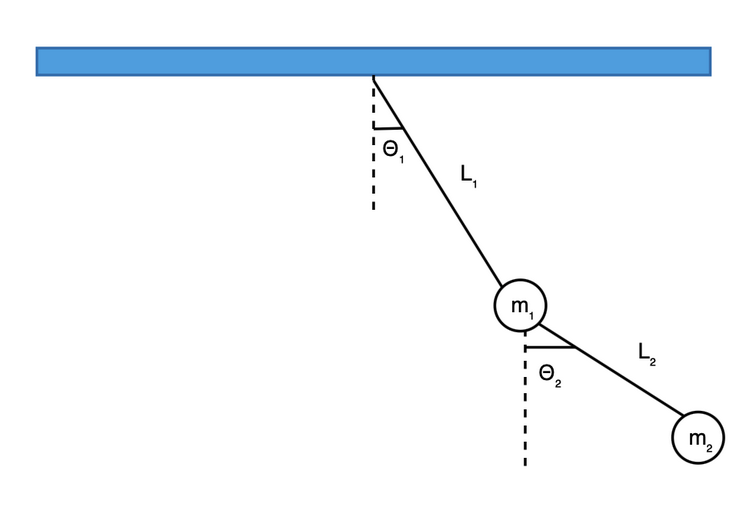
\includegraphics[width=0.6\textwidth]{figures/DblPendulum.png}
  \caption{Double Pendulum Demonstration}
  \label{fig_dblpen}
\end{figure}

\begin{table}[ht]
	\begin{tabular}{ p{0.2\textwidth} p{0.7\textwidth} }
		\textbf{Name} & \textbf{Description} \\
		\toprule
		\verb|m₁| & The mass of the first object\\
    \verb|m₂| & The mass of the second object\\
		\verb|L₁| & The length of the first rod\\
		\verb|L₂| & The length of the second rod\\
		\verb|g| & Gravitational acceleration\\
		\verb|θ₁| & The angle of the first rod\\
		\verb|θ₂| & The angle of the second rod\\
		\verb|ω₁| & The angular velocity of the first object\\
		\verb|ω₂| & The angular velocity of the second object\\
		\bottomrule	
	\end{tabular}	
	\caption{Variables in Double Pendulum Example}	
	\label{tab_dblpendes}
\end{table}

This point we have primarily focusing on solving linear ODEs. However, despite the \href{https://jacquescarette.github.io/Drasil/examples/dblpendulum/SRS/srs/DblPendulum_SRS.html#Sec:IMs}{Double Pendulum case study} containing a non-linear ODE, the Drasil framework can still generate code to solve it numerically with some additional help from the user. 

In the Double Pendulum case study, we want to solve the following equations:
\begin{flalign} \label{eq_dblpenhigh}
  & \theta_{1}'' = \frac{-g(2m_{1}+m_{2})\sin \theta_{1}-m_{2}g\sin (\theta_{1}-2\theta_{2})-2\sin (\theta_{1}-\theta_{2})m_{2}({\theta_{2}'}^2L_{2}+{\theta_{1}'}^2L_{1}\cos (\theta_{1}-\theta_{2}))}{L_{1}(2m_{1}+m_{2}-m_{2}\cos (2\theta_{1}-2\theta_{2}))} \\ \nonumber
  & \theta_{2}'' = \frac{2\sin (\theta_{1}-\theta_{2})({\theta_{1}'}^2L_{1}(m_{1}+m_{2})+g(m_{1}+m_{2})\cos \theta_{1} + {\theta_{2}'}^2L_{2}m_{2}\cos (\theta_{1}-\theta_{2}))}{L_{2}(2m_{1}+m_{2}-m_{2}\cos (2\theta_{1}-2\theta_{2}))}
\end{flalign}
\myequations{Double Pendulum Equation}
There are two second-order ODEs in one system. To solve this system of ODEs, we convert them into a system of first-order ODEs. The transformation follows the methodology we discussed in Section~\ref{se_hightofirst}. We transform Equation~\ref{eq_dblpenhigh} into Equation~\ref{eq_dblpenfirst}. Once the transformation is complete, we can encode Equation~\ref{eq_dblpenfirst} and pass it to the Drasil Code Generator. However, we cannot show Equation~\ref{eq_dblpenfirst} in the shape of Equation~\ref{eq_foode} because the ODE is not a linear ODE.

\begin{flalign} \label{eq_dblpenfirst}
  & \theta_{1}' = \omega_{1} \\ \nonumber
  & \theta_{2}' = \omega_{2} \\ \nonumber
  & \omega_{1}' = \frac{-g(2m_{1}+m_{2})\sin \theta_{1}-m_{2}g\sin (\theta_{1}-2\theta_{2})-2\sin (\theta_{1}-\theta_{2})m_{2}({\omega{2}}^2L_{2}+{\omega{1}}^2L_{1}\cos (\theta_{1}-\theta_{2}))}{L_{1}(2m_{1}+m_{2}-m_{2}\cos (2\theta_{1}-2\theta_{2}))} \\ \nonumber
  & \omega_{2}' = \frac{2\sin (\theta_{1}-\theta_{2})({\omega_{1}}^2L_{1}(m_{1}+m_{2})+g(m_{1}+m_{2})\cos \theta_{1} + {\omega_{2}}^2L_{2}m_{2}\cos (\theta_{1}-\theta_{2}))}{L_{2}(2m_{1}+m_{2}-m_{2}\cos (2\theta_{1}-2\theta_{2}))}
\end{flalign}
\myequations{Double Pendulum Equation in a System of First-Order ODEs}

Now that we have obtained Equation~\ref{eq_dblpenfirst}, we can encode it in Drasil. Code~\ref{code_encodedblpend} shows the example of how we encode Equation~\ref{eq_dblpenfirst} in the Drasil. We replace the Drasil language with mathematical symbols to increase the readability of the code.
\begin{listing}[ht]
\begin{haskell1}
dblPenODEInfo :: ODEInfo
dblPenODEInfo = odeInfo
...
[3*π/7, 0, 3*π/4, 0] -- initial values
[ ω₁,
  -g(2m₁ + m₂)sin θ₁ - m₂gsin (θ₁ - 2θ₂) - 2sin (θ₁ - θ₂)m₂(ω₂²L₂ + ω₁²L₁cos (θ₁ - θ₂)) / L₁(2m₁ + m₂ -m₂cos (2θ₁ - 2θ₂)),
  ω₂,
  2sin (θ₁ - θ₂)(ω₁²L₁(m₁ + m₂ ) + g(m₁ + m₂ )cos θ₁ + ω₂²L₂m₂cos (θ₁ - θ₂ )) / L₂(2m₁ + m₂ -m₂cos (2θ₁ - 2θ₂))
]
...
\end{haskell1}
\captionof{listing}{Pseudocode for Encoding Double Pendulum's Equation}
\label{code_encodedblpend}
\end{listing}

Once the \verb|dblPenODEInfo| is ready, we will pass it to the Drasil Code generator. It will generate code to solve the Double Pendulum in four languages. The details of the generated code are in Appendix~\ref{gencodedbl}. However, the Double Pendulum case study cannot utilize any function introduced in the next section because they were designed for a linear ODE.

The limitation of manually creating \verb|ODEInfo| is that we will write the ODE twice in different ways. In this case, we encode both Equation~\ref{eq_dblpenhigh} and Equation~\ref{eq_dblpenfirst} in Drasil. They both demonstrate the same phenomena and exist in an isomorphic ODE type. The following section will discuss how to automate the transformation from a higher-order linear ODE to a system of first-order ODEs.

\section{Generate ODEInfo Automatically}
Manually creating explicit equations is not ideal because it requires human interference and propagates duplicate information. We want to design the Drasil framework to be as fully automatic as possible. Therefore, an ideal solution is to encode the ODE in a flexible data structure. Then, we can extract information from this structure and generate a form of the ODE that selected external libraries can utilize. Creating the \verb|DifferentialModel| data structure satisfies the need of this idea for linear ODEs. We can restructure an ODE based on the information from \verb|DifferentialModel|. This research's scope only covers generating explicit equations for a single higher-order linear ODE. In the future, we want to generate explicit equations for a system of higher-order ODEs and nonlinear ODEs.

Once we encode the ODE in \verb|DifferentialModel|, we want to restructure its equivalent system of first-order ODEs in the shape of Equation~\ref{eq_foode}. For the convenience of implementation, we shuffle the data around in Equation~\ref{eq_foodeexample}. We reverse the order of $\boldsymbol{x}$ to $x_{n}$, $\dots$, $x_{1}$. The coefficient matrix $\boldsymbol{A}$ also changes, but $\boldsymbol{x'}$ and $\boldsymbol{c}$ remain unchanged.

\begin{equation} \label{eq_foodeexamplecolor}
	\begin{bmatrix}
		\highlight{yellow}{x_{1}'} \\
    \highlight{yellow}{\dots} \\
    \highlight{yellow}{x_{n-2}'} \\
    \highlight{yellow}{x_{n-1}'} \\
    \highlight{yellow}{x_{n}'}
	\end{bmatrix}
    = 
  \begin{bmatrix}
		\highlight{orange}{0}, & \highlight{orange}{0}, & \highlight{orange}{\dots}, & \highlight{orange}{1}, & \highlight{orange}{0} \\
    \highlight{orange}{\dots} \\
    \highlight{orange}{0}, & \highlight{orange}{1}, & \highlight{orange}{\dots}, & \highlight{orange}{0}, & \highlight{orange}{0} \\
    \highlight{orange}{1}, & \highlight{orange}{0}, & \highlight{orange}{\dots}, & \highlight{orange}{0}, & \highlight{orange}{0} \\
    \highlight{cyan}{b_{n-1}(t)}, & \highlight{cyan}{b_{n-2}(t)}, & \highlight{cyan}{\dots}, & \highlight{cyan}{b_{1}(t)}, & \highlight{cyan}{b_{0}(t)}
	\end{bmatrix}
    \cdot
  \begin{bmatrix}
    \highlight{yellow}{x_{n}} \\
    \highlight{yellow}{\dots} \\
    \highlight{yellow}{x_{3}} \\
		\highlight{yellow}{x_{2}} \\
    \highlight{yellow}{x_{1}}
	\end{bmatrix}
    + 
  \begin{bmatrix}
    \highlight{lightgray}{0} \\
    \highlight{lightgray}{0} \\
    \highlight{lightgray}{\dots} \\
    \highlight{lightgray}{0} \\
    \highlight{red}{h(t)}
	\end{bmatrix}
\end{equation}

Since Equation~\ref{eq_foodeexamplecolor} is an expansion of Equation~\ref{eq_foode}, we will use symbols in both equations to explain how to generate Equation~\ref{eq_foodeexamplecolor}. We highlighted $\boldsymbol{x'}$ and $\boldsymbol{x}$ in yellow in Equation~\ref{eq_foodeexamplecolor}. The number of elements in $\boldsymbol{x'}$ and $\boldsymbol{x}$ depends on how many new dependent variables are introduced. If the higher-order ODE is second-order, we will introduce two new dependent variables. If the higher-order ODE is $n^{th}$-order, we will introduce $n$ new dependent variables. For $\boldsymbol{x'}$, knowing it is $n^{th}$-order ODE, we parameterize $x'_{1}, \dots, x'_{n}$. For $\boldsymbol{x}$, knowing it is $n^{th}$-order ODE, we parameterize $x_{n}, \dots, x_{1}$.

We highlighted the $n \times n$ coefficient matrix $\boldsymbol{A}$ in orange and blue in Equation~\ref{eq_foodeexamplecolor}. The orange part is a matrix that looks like the identity matrix, only rotated and with an extra column of 0s. For the lowest higher-order ODE, a second-order ODE, the orange part is $[1, 0]$. Equation~\ref{eq_foodeexamplecolortwo} shows a completed transformation for a second-order linear ODE.
\begin{equation} \label{eq_foodeexamplecolortwo}
	\begin{bmatrix}
		{x_{1}'} \\
    {x_{2}'} 
	\end{bmatrix}
    = 
  \begin{bmatrix}
		\highlight{orange}{1}, & \highlight{orange}{0} \\
    {b_{1}(t)}, & {b_{0}(t)}
	\end{bmatrix}
    \cdot
  \begin{bmatrix}
		{x_{2}} \\
    {x_{1}} 
	\end{bmatrix}
    + 
  \begin{bmatrix}
    {0} \\
    {h(t)}
	\end{bmatrix}
\end{equation}

The $\boldsymbol{A}$ will be a $4 \times 4$ matrix for a fourth-order ODE. Equation~\ref{eq_foodeexamplecolorfour} shows a completed transformation for a fourth-order ODE.
\begin{equation} \label{eq_foodeexamplecolorfour}
	\begin{bmatrix}
		{x_{1}'} \\
    {x_{2}'} \\
    {x_{3}'} \\
    {x_{4}'}
	\end{bmatrix}
    = 
  \begin{bmatrix}
		\highlight{orange}{0}, & \highlight{orange}{0}, & \highlight{orange}{1}, & \highlight{orange}{0} \\
    \highlight{orange}{0}, & \highlight{orange}{1}, & \highlight{orange}{0}, & \highlight{orange}{0} \\
    \highlight{orange}{1}, & \highlight{orange}{0}, & \highlight{orange}{0}, & \highlight{orange}{0} \\
    {b_{3}(t)}, & {b_{2}(t)}, & {b_{1}(t)}, & {b_{0}(t)}
	\end{bmatrix}
    \cdot
  \begin{bmatrix}
		{x_{4}} \\
    {x_{3}} \\
    {x_{2}} \\
    {x_{1}}
	\end{bmatrix}
    + 
  \begin{bmatrix}
    {0} \\
    {0} \\
    {0} \\
    {h(t)}
	\end{bmatrix}
\end{equation}

The orange part starts at the ${n-1}^{th}$ row with $[1, 0, \dots]$. If there is a second row, we add $[0, 1, \dots]$ above the start row and so on. We observe a pattern for the orange part so that we can generate it. In Code~\ref{code_createidentity}, \verb|constIdentityRowVect| and \verb|addIdentityValue| are responsible for generating each row in the orange part. We first create a row containing a list of 0. Then, we replace one of the 0s with 1. The \verb|addIdentityCoeffs| run through a recursion that combines all rows to form the orange and blue parts.

\begin{listing}
\begin{haskell1}
-- | Add Identity Matrix to Coefficients
-- | len is the length of the identity row,
-- | index is the location of identity value (start with 0)
addIdentityCoeffs :: [[Expr]] -> Int -> Int -> [[Expr]]
addIdentityCoeffs es len index
  | len == index + 1 = es
  | otherwise = addIdentityCoeffs (constIdentityRowVect len index : es) len (index + 1)

-- | Construct an identity row vector.
constIdentityRowVect :: Int -> Int -> [Expr]
constIdentityRowVect len index = addIdentityValue index $ replicate len $ exactDbl 0

-- | Recreate the identity row vector with identity value 
addIdentityValue :: Int -> [Expr] -> [Expr]
addIdentityValue n es = fst splits ++ [exactDbl 1] ++ tail (snd splits)
  where splits = splitAt n es
\end{haskell1}
\captionof{listing}{Source Code for Creating Identity Matrix (Highlighted in Orange)}
\label{code_createidentity}
\end{listing}

We highlighted the constant vector $\boldsymbol{c}$ in gray and red colour in Equation~\ref{eq_foodeexamplecolor}. The vector $\boldsymbol{c}$ has the length $n$. The last element of the constant vector $\boldsymbol{c}$ will be $h(t)$, and anything above $h(t)$ will be 0. In Code~\ref{code_createconstant}, in \verb|addIdentityConsts|, given the expression of $[h(t)]$ and the order number of the ODE, we add $(n-1)$ 0s above the $h(t)$. 

\begin{listing}
\begin{haskell1}
-- | Add zeros to Constants
-- | len is the size of new constant vector
addIdentityConsts :: [Expr] -> Int -> [Expr]
addIdentityConsts expr len = replicate (len - 1) (exactDbl 0) ++ expr
\end{haskell1}
\captionof{listing}{Source Code for Creating Constant Matrix}
\label{code_createconstant}
\end{listing}

The blue and red parts in Equation~\ref{eq_foodeexamplecolor} can be determined by Equation~\ref{eq_linearDE}. The \verb|DifferentialModel| captures the relationship for Equation~\ref{eq_linearDE} but does not isolate the highest order to the left-hand side. To isolate the highest order, we have to shuffle terms between the left-hand side and right-hand side. The following is a demonstration of how to create the blue part. Giving the following equation:
\begin{equation}
	a_n(t) \cdot y^n(t) + a_{n-1}(t) \cdot y^{\textit{(n-1)}}(t) + \dots + a_1(t) \cdot y'(t) + a_0(t) \cdot y(t) = h(t) \nonumber
\end{equation}
Firstly, we move every term from left to right, except the highest order term. 
\begin{equation}
	a_n(t) \cdot y^n(t)  = -a_{n-1}(t) \cdot y^{\textit{(n-1)}}(t) + \dots + -a_1(t) \cdot y'(t) + -a_0(t) \cdot y(t) + h(t) \nonumber
\end{equation}
Secondly, we divide both sides of the equation by the coefficient $a_n(t)$.
\begin{equation}
	y^n(t)  = \frac{-a_{n-1}(t) \cdot y^{\textit{(n-1)}}(t) + \dots + -a_1(t) \cdot y'(t) + -a_0(t) \cdot y(t) + h(t)}{a_n(t)} \nonumber
\end{equation}
Then, we can write this in matrix form as:
\begin{equation} 
  \begin{bmatrix}
		y^n(t)
	\end{bmatrix}
  = 
	\begin{bmatrix}
		-\frac{a_{n-1}(t)}{a_n(t)}, \dots, & -\frac{a_{1}(t)}{a_n(t)} & -\frac{a_{0}(t)}{a_n(t)}
	\end{bmatrix}
	\cdot
	\begin{bmatrix}
		y^{\textit{(n-1)}}(t) \\
		\dots \\
    y'(t) \\
		y(t)  
	\end{bmatrix}
	+
	\begin{bmatrix}
		\frac{h(t)}{a_n(t)}
	\end{bmatrix}
  \nonumber
\end{equation}
Since $x_{n}'$ = $y_{n}$ (Equation~\ref{eq_diffvervars}), we can replace $y_{n}$ with $x_{n}'$. Based on Equation~\ref{eq_newvars}, we replace all derivatives of $y(t)$ with $x_{n}, \dots, x_{1}$.

\begin{equation}
  \begin{bmatrix}
		x_{n}'
	\end{bmatrix}
  = 
	\begin{bmatrix}
		-\frac{a_{n-1}(t)}{a_n(t)}, \dots, & -\frac{a_{1}(t)}{a_n(t)} & -\frac{a_{0}(t)}{a_n(t)}
	\end{bmatrix}
	\cdot
	\begin{bmatrix}
		x_{n} \\
		\dots \\
    x_{2} \\
		x_{1}  
	\end{bmatrix}
	+
	\begin{bmatrix}
		\frac{h(t)}{a_n(t)}
	\end{bmatrix}
  \nonumber
\end{equation}
Lastly, we replace new variables in Equation~\ref{eq_foodeexamplecolor} to get a new matrix.
\begin{equation}\label{eq_foodeexampledetail}
	\begin{bmatrix}
		\highlight{yellow}{x_{1}'} \\
    \highlight{yellow}{\dots} \\
    \highlight{yellow}{x_{n-2}'} \\
    \highlight{yellow}{x_{n-1}'} \\
    \highlight{yellow}{x_{n}'}
	\end{bmatrix}
    = 
  \begin{bmatrix}
		\highlight{orange}{0}, & \highlight{orange}{0}, & \highlight{orange}{\dots}, & \highlight{orange}{1}, & \highlight{orange}{0} \\
    \highlight{orange}{\dots} \\
    \highlight{orange}{0}, & \highlight{orange}{1}, & \highlight{orange}{\dots}, & \highlight{orange}{0}, & \highlight{orange}{0} \\
    \highlight{orange}{1}, & \highlight{orange}{0}, & \highlight{orange}{\dots}, & \highlight{orange}{0}, & \highlight{orange}{0} \\
    \highlight{cyan}{-\frac{a_{n-1}(t)}{a_n(t)}}, & \highlight{cyan}{-\frac{a_{n-2}(t)}{a_n(t)}}, & \highlight{cyan}{\dots}, & \highlight{cyan}{-\frac{a_{1}(t)}{a_n(t)}}, & \highlight{cyan}{-\frac{a_{0}(t)}{a_n(t)}}
	\end{bmatrix}
    \cdot
  \begin{bmatrix}
    \highlight{yellow}{x_{n}} \\
    \highlight{yellow}{\dots} \\
    \highlight{yellow}{x_{3}} \\
		\highlight{yellow}{x_{2}} \\
    \highlight{yellow}{x_{1}}
	\end{bmatrix}
    + 
  \begin{bmatrix}
    \highlight{lightgray}{0} \\
    \highlight{lightgray}{0} \\
    \highlight{lightgray}{\dots} \\
    \highlight{lightgray}{0} \\
    \highlight{red}{\frac{h(t)}{a_n(t)}}
	\end{bmatrix}
\end{equation}
\myequations{Expansion of System of First-Order ODEs in Matrix Form}

Here is the implementation for creating Equation~\ref{eq_foodeexampledetail} in Drasil. In Code~\ref{code_isohighode}, we remove the highest order because we want to isolate the highest order to the left-hand side.
\begin{listing}[ht]
\begin{haskell1}
-- | Delete the highest order
transUnknowns :: [Unknown] -> [Unknown]
transUnknowns = tail
\end{haskell1}
\captionof{listing}{Source Code for Isolating the Highest Order}
\label{code_isohighode}
\end{listing}

In Code~\ref{code_cancelcoe}, the \verb|transCoefficients| divide the coefficient $a_n(t)$ in blue highlighted. The \verb|divideConstants| divide the coefficient in the red highlights.
\begin{listing}[ht]
\begin{haskell1}
-- | Cancel the leading coefficient of the highest order in the coefficient matrix
transCoefficients :: [Expr] -> [Expr]
transCoefficients es
  | head es == exactDbl 1 = mapNeg $ tail es
  | otherwise = mapNeg $ tail $ map ($/ head es) es
    where mapNeg = map (\x -> if x == exactDbl 0 then exactDbl 0 else neg x)

-- | divide the leading coefficient of the highest order in constant
divideConstants :: Expr -> Expr -> Expr
divideConstants a b
  | b == exactDbl 0 = error "Divisor can't be zero"
  | b == exactDbl 1 = a
  | otherwise       = a $/ b
\end{haskell1}
\captionof{listing}{Source Code for Canceling the Coefficient from the Highest Order}
\label{code_cancelcoe}
\end{listing}

In Code~\ref{code_odesolverformat}, we create a new \verb|data type| called \verb|ODESolverFormat|. The \verb|ODESolverFormat| contains information for the system of first-order ODEs. The \verb|coeffVects|, \verb|unknownVect|, and \verb|constantVect| are responsible for $\boldsymbol{A}$, $\boldsymbol{x}$, and $\boldsymbol{c}$ in Equation~\ref{eq_foode}. The \verb|makeAODESolverFormat| is a smart constructor to create an \verb|ODESolverFormat| by providing a \verb|DifferentialModel|.

\begin{listing}
\begin{haskell1}
-- Acceptable format for ODE solvers
-- X' = AX + c
-- coeffVects is A - coefficient matrix with identity matrix
-- unknownVect is X - unknown column vector after reduce the highest order
-- constantVect is c - constant column vector with identity matrix, 
-- X' is a column vector of first-order unknowns
data ODESolverFormat = X'{
  coeffVects :: [[Expr]],
  unknownVect :: [Integer],
  constantVect :: [Expr]
}

-- | Construct an ODESolverFormat for solving the ODE.
makeAODESolverFormat :: DifferentialModel -> ODESolverFormat
makeAODESolverFormat dm = X' transEs transUnks transConsts
  where transUnks = transUnknowns $ dm ^. unknowns
        transEs = addIdentityCoeffs [transCoefficients $ head (dm ^. coefficients)] (length transUnks) 0
        transConsts = addIdentityConsts [head (dm ^. dmConstants) `divideCosntants` head (head (dm ^. coefficients))] (length transUnks)
\end{haskell1}
\captionof{listing}{Source Code for Generating Equation~\ref{eq_foode}}
\label{code_odesolverformat}
\end{listing}

In Chapter 3 we mentioned we would solve the ODE as an IVP. In Code~\ref{code_ivpinfo}, we create \verb|InitialValueProblem| to store IVP-related information, including initial time, the final time and initial values.
\begin{listing}
\begin{haskell1}
-- Information for solving an initial value problem
data InitialValueProblem = IVP{
  initTime :: Expr, -- inital time
  finalTime :: Expr, -- end time
  initValues :: [Expr] -- initial values
}
\end{haskell1}
\captionof{listing}{Source Code for IVP Infomation}
\label{code_ivpinfo}
\end{listing}

Lastly, in Code~\ref{code_generateodeinfo}, we create a new smart constructor to generate the \verb|ODEInfo| automatically. In \verb|odeInfo'|, the first parameter is \verb|[CodeVarChunk]|. There will likely be other variables in the ODE. The \verb|[CodeVarChunk]| contains variable parameters other than the dependent and independent variables. The \href{https://jacquescarette.github.io/Drasil/docs/full/drasil-code-0.1.9.0/Language-Drasil-Data-ODEInfo.html#t:ODEOptions}{ODEOptions} instructs the Drasil Code Generator on how external libraries solve the ODE. The \verb|DifferentialModel| contains core information for the higher-order ODE. Lastly, the \verb|InitialValueProblem| contains information for solving the ODEs numerically. The \verb|createFinalExpr| creates multiple expressions in a list. Those expressions were created based on information on the system of first-order ODEs. The \verb|formEquations| take the following parameters: the coefficient matrix $\boldsymbol{A}$ (\verb|[[Expr]]|), the unknown vector $\boldsymbol{x}$ (combining \verb|[Unknown]| and \verb|ConstrConcept|), and the constant vector $\boldsymbol{c}$ (\verb|[Expr]|). Those parameters contain enough information to create explicit equations for the Drasil Code Generator. We can create explicit equations by taking the dot product of $\boldsymbol{A}$ and $\boldsymbol{x}$, and then adding the constant term. The \verb|formEquations| will output a list of expressions equivalent to Equation~\ref{eq_diffvervarslinear}. Once explicit equations for the higher-order ODE are created, we can pass it to the Drasil Code Generator.

\begin{listing}[ht]
\begin{haskell1}
odeInfo' :: [CodeVarChunk] -> ODEOptions -> DifferentialModel -> InitialValueProblem -> ODEInfo
odeInfo' ovs opt dm ivp = ODEInfo 
  (quantvar $ _indepVar dm) 
  (quantvar $ _depVar dm) 
  ovs 
  (expr $ initTime ivp)
  (expr $ finalTime ivp)
  (map expr $ initValues ivp)
  (createFinalExpr dm)
  opt

createFinalExpr :: DifferentialModel -> []
createFinalExpr dm = map expr $ formEquations (coeffVects ode) (unknownVect ode) (constantVect ode) (_depVar dm)
  where ode = makeAODESolverFormat dm

formEquations :: [[Expr]] -> [Unknown] -> [Expr] -> ConstrConcept-> [Expr]
formEquations [] _ _ _ = []
formEquations _ [] _ _ = []
formEquations _ _ [] _ = []
formEquations (ex:exs) unks (y:ys) depVa =
  (if y == exactDbl 0 then finalExpr else finalExpr `addRe` y) : formEquations exs unks ys depVa
  where indexUnks = map (idx (sy depVa) . int) unks -- create X
        filteredExprs = filter (\x -> fst x /= exactDbl 0) (zip ex indexUnks) -- remove zero coefficients
        termExprs = map (uncurry mulRe) filteredExprs -- multiple coefficient with depend variables
        finalExpr = foldl1 addRe termExprs -- add terms together
\end{haskell1}
\captionof{listing}{Source Code for Generating ODEInfo}
\label{code_generateodeinfo}
\end{listing}
